\documentclass[12pt]{beamer}

\usetheme{Oxygen}
\usepackage[spanish]{babel}
\usepackage{thumbpdf}
\usepackage{wasysym}
\usepackage{ucs}
\usepackage[utf8]{inputenc}
\usepackage{pgf,pgfarrows,pgfnodes,pgfautomata,pgfheaps,pgfshade}
\usepackage{verbatim}
\usenavigationsymbolstemplate{}

\pdfinfo
{
  /Title       (KPARTS)
  /Creator     (KILE)
  /Author      (RAFAEL FERNANDEZ LOPEZ)
}

\AtBeginSection[]
{
  \frame<handout:0>
  {
    \frametitle{Akademy-es 2008}
    \tableofcontents[currentsection]
  }
}

\title{KParts}
\subtitle{Una introducción a KParts}
\author{Rafael Fernández López}
\date{Noviembre, 2008}

\begin{document}

\begin{frame}{Akademy-es 2008}
  \framesubtitle{ereslibre@kde.org}
  \titlepage
\end{frame}


\section*{}
\begin{frame}{Akademy-es 2008}
  \framesubtitle{}
  \tableofcontents[section=1]
\end{frame}

\newcommand<>{\highlighton}[1]{%
  \alt#2{\structure{#1}}{{#1}}
}

\newcommand{\icon}[1]{\pgfimage[height=1em]{#1}}


\section{Un poco de historia}

\begin{frame}{Un poco de historia}
  \framesubtitle{XmlGui y KParts}
  \begin{itemize}
    \item KParts se hizo público en la rama de KDE 2, hace unos 7 años
    \item XmlGui ya existía por aquel entonces (se comenzó en 1997 aproximadamente)
    \item Código muy estable
    \item Debido a grandísimos cambios en Qt, el código ha ido evolucionando, quedando algunos
          ``restos'' que todavía tienen que ser pulidos
    \item Mejorable a día de hoy
    \begin{itemize}
      \item Tests automatizados → fundamentales (QTestLib)
      \begin{itemize}
        \item \textit{Give me a way to break it and I will find a way to fix it}
      \end{itemize}
    \end{itemize}
    \item Principal consumidor
    \begin{itemize}
      \item Konqueror
    \end{itemize}
  \end{itemize}
\end{frame}


\section{Introducción a XmlGui}

\begin{frame}{¿Qué es XmlGui?}
  \framesubtitle{}
  \begin{itemize}
    \item Framework para desarrolladores
    \item Objetivos:
      \begin{itemize}
        \item Definir interfaces gráficas de usuario mediante ficheros con estructura XML
          \begin{itemize}
            \item Consistencia
          \end{itemize}
        \item Modificar ``en caliente'' la interfaz de una aplicación o un componente
          \begin{itemize}
            \item Cambio de acciones en una barra de herramientas
          \end{itemize}
        \item Permitir cargar componentes que amplíen la interfaz de origen
          \begin{itemize}
            \item Plugins
          \end{itemize}
        \item Estructura bien definida mediante ficheros DTD
      \end{itemize}
  \end{itemize}
\end{frame}


\section{KParts}

\subsection{Objetivos}

\subsubsection{Cliente}

\begin{frame}{Objetivos del cliente (1)}
  \framesubtitle{}
  En general, hay dos tipos de clientes:
  \medskip
  \begin{itemize}
    \item Leer uno o varios tipos de ficheros determinados
    \begin{itemize}
      \item Mejora la experiencia del usuario de manera muy focal
      \item Se centra en un servicio determinado propocionado por un componente determinado
      \item Se conoce de antemano qué tipo de fichero tratará de leerse de manera embebida
      \begin{itemize}
        \item { \alert{Importante:} se conocerá en tiempo de ejecución si es posible leerlo }
      \end{itemize}
    \end{itemize}
    \smallskip
    \begin{block}{Ejemplo}
      Administrador de documentos científicos. Podría preguntar al sistema si existe algún servicio
      de lectura de ficheros que soporte el formato PDF
    \end{block}
  \end{itemize}
\end{frame}

\begin{frame}{Objetivos del cliente (2)}
  \framesubtitle{}
  \begin{itemize}
    \item Leer el máximo número de tipos de ficheros posible
      \begin{itemize}
        \item Proporcionar al usuario la máxima comodidad posible
        \item Permite maximizar la multitud de tipos de ficheros distintos sin abrir una aplicación
              separada
      \end{itemize}
      \medskip
      \begin{block}{Ejemplo}
        Konqueror. Si está configurado para ello, cuando se le solicite abrir un fichero, tratará
        de embeberlo si hay algún componente que sabe leerlo. En caso contrario, lanzará la
        aplicación encargada de ese tipo de fichero
      \end{block}
  \end{itemize}
\end{frame}

\begin{frame}{Objetivos del cliente (3)}
 \framesubtitle{}
 Ambos consiguen:
 \medskip
 \begin{itemize}
   \item Se benefician de las mejoras que se hagan en el componente automáticamente
   \item Mejoran la navegación
   \begin{itemize}
     \item El componente que provee el servicio es ``embebido'' en la aplicación contenedora
   \end{itemize}
   \item Evita duplicar código
 \end{itemize}
\end{frame}

\subsubsection{Servicio}

\begin{frame}{Objetivos del servicio}
  \framesubtitle{}
  \begin{itemize}
    \item Ofrecer una funcionalidad muy específica e independiente del contexto
    \begin{itemize}
      \item Añadir menús
      \item Añadir acciones a una (o varias) barra(s) de herramientas
      \item Ofrecer sus propias barras de herramientas
      \item Éste a su vez podría ser ampliado mediante plugins
    \end{itemize}
  \end{itemize}
  \begin{itemize}
    \item ¿Merece la pena escribir un servicio? Depende:
    \begin{itemize}
      \item Es incorrecta la idea de escribir un servicio exportando un widget
        \begin{itemize}
          \item En este sentido ya contamos con las librerías de siempre
          \item Merece la pena crear un servicio que exporte una funcionalidad relativamente
                compleja, que posiblemente, lea tipos de ficheros que no sean soportados por otras
                aplicaciones, aunque esto no es un requerimiento forzoso
        \end{itemize}
    \end{itemize}
  \end{itemize}
\end{frame}

\subsection{Estructura}

\begin{frame}{Estructura}
  \framesubtitle{}
  \begin{center}
    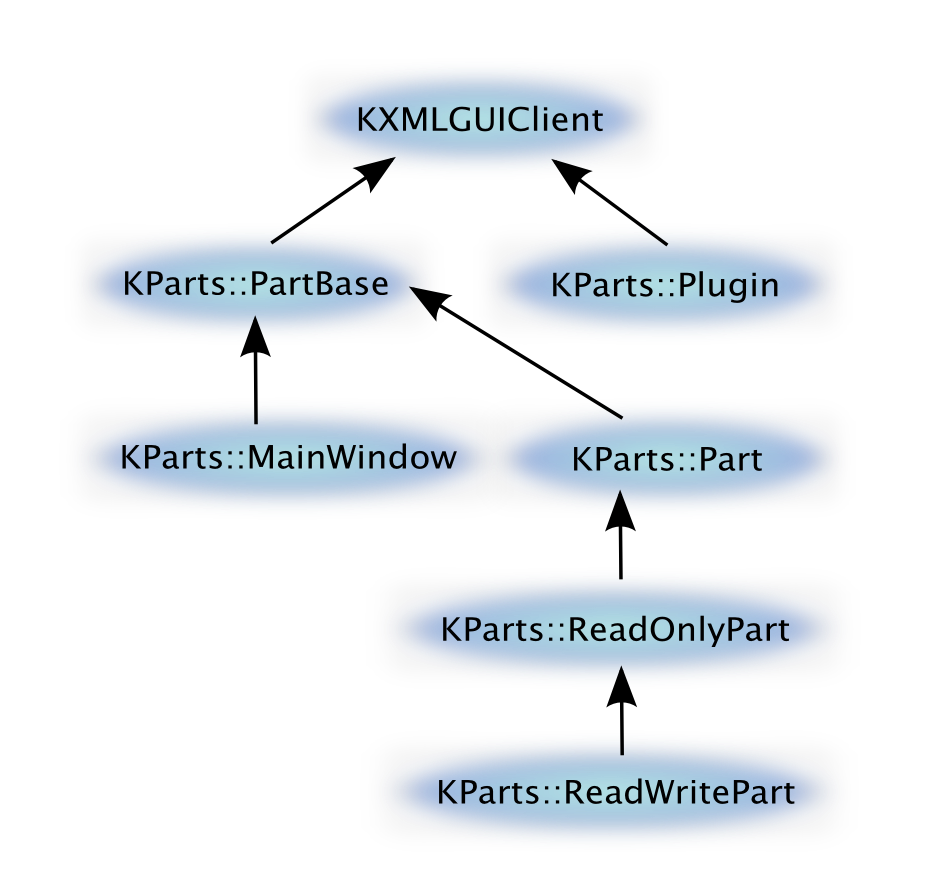
\includegraphics[width=200px,height=200px]{esquema.png}
  \end{center}
\end{frame}

\frame{
  \frametitle{Akademy-es 2008}
  \vspace{1.5cm}
  {\huge \alert{\textbf{Gracias.}} ¿Preguntas?}

  \vspace{3.5cm}
  \begin{flushright}
    Rafael Fernández López

    \structure{\footnotesize{ereslibre@kde.org}}
  \end{flushright}
}

\end{document}
